\documentclass[11pt]{report}
\usepackage[margin=1in]{geometry}
\usepackage{amsfonts,amsmath,amssymb}
\usepackage[italian]{babel}
\usepackage{fancyhdr}

\usepackage{pgfplots} %grafici e colori
\usepackage{xcolor}
\usepackage{tikz}

\usepackage{graphicx} %figure
\usepackage{wrapfig}

\usepackage{isotope} %equazioni chimiche

\usetikzlibrary{ shapes.geometric } %liberie tikz
\usetikzlibrary{calc}
\usepackage{anyfontsize}
\pgfplotsset{width=10cm,compat=1.9}

\title{DNA}
\author{Tommaso Severini}

\pagestyle{fancy}
\fancyhead{}
\fancyfoot{}
\fancyhead[L]{DNA}
\fancyhead[R]{Tommaso Severini}
\fancyfoot[C]{\thepage}

\parindent 0ex

\begin{document}
	
	\begin{titlepage}
		\pagestyle{empty}
		
		\begin{tikzpicture}[remember picture,overlay]
			%%%%%%%%%%%%%%%%%%%% Background %%%%%%%%%%%%%%%%%%%%%%%%
			\fill[red] (current page.south west) rectangle (current page.north east);
			
			
			\foreach \i in {2.5,...,22}
			{
				\node[rounded corners,red!60,draw,regular polygon,regular polygon sides=6, minimum size=\i cm,ultra thick] at ($(current page.west)+(2.5,-5)$) {} ;
			}
			
			%%%%%%%%%%%%%%%%%%%% Background Polygon %%%%%%%%%%%%%%%%%%%% 
			\foreach \i in {0.5,...,22}
			{
				\node[rounded corners,red!60,draw,regular polygon,regular polygon sides=6, minimum size=\i cm,ultra thick] at ($(current page.north west)+(2.5,0)$) {} ;
			}
			
			\foreach \i in {0.5,...,22}
			{
				\node[rounded corners,red!90,draw,regular polygon,regular polygon sides=6, minimum size=\i cm,ultra thick] at ($(current page.north east)+(0,-9.5)$) {} ;
			}
			
			
			\foreach \i in {21,...,6}
			{
				\node[red!85,rounded corners,draw,regular polygon,regular polygon sides=6, minimum size=\i cm,ultra thick] at ($(current page.south east)+(-0.2,-0.45)$) {} ;
			}
			
			
			%%%%%%%%%%%%%%%%%%%% Title of the Report %%%%%%%%%%%%%%%%%%%% 
			\node[left,red!5,minimum width=0.625*\paperwidth,minimum height=3cm, rounded corners] at ($(current page.north east)+(0,-9.5)$)
			{
				{\fontsize{25}{30} \selectfont \bfseries DNA}
			};
			
			%%%%%%%%%%%%%%%%%%%% Subtitle %%%%%%%%%%%%%%%%%%%% 
			\node[left,red!10,minimum width=0.625*\paperwidth,minimum height=2cm, rounded corners] at ($(current page.north east)+(0,-11)$)
			{
				{\huge \textit{Da Griffith al progetto Genoma Umano}}
			};
			
			%%%%%%%%%%%%%%%%%%%% Author Name %%%%%%%%%%%%%%%%%%%% 
			\node[left,red!5,minimum width=0.625*\paperwidth,minimum height=2cm, rounded corners] at ($(current page.north east)+(0,-13)$)
			{
				{\Large \textsc{Tommaso Severini}}
			};
			
			%%%%%%%%%%%%%%%%%%%% Year %%%%%%%%%%%%%%%%%%%% 
			\node[rounded corners,fill=red!70,text =red!5,regular polygon,regular polygon sides=6, minimum size=2.5 cm,inner sep=0,ultra thick] at ($(current page.west)+(2.5,-5)$) {\LARGE \bfseries 2021};
			
		\end{tikzpicture}
	\end{titlepage}	
	
	\chapter{La scoperta e le sue tappe più importanti}
	
	L'alterazione delle caratteristiche ereditarie delle cellule è un'operazione compiuta quotidianamente nei laboratori oggigiorno, ma, agli inizi del XX secolo, non era ancora nota l'identità del materiale genetico. Nonostante ciò, la comunità scientifica dell'epoca era a conoscenza del fatto che i cromosomi fossero responsabili del trasporto delle informazioni ereditarie. Perciò rimaneva solo da capire quale dei componenti chimici dei cromosomi trasportassero le informazioni genetiche: il DNA o le proteine. Contrariamente alle conoscenze moderne, fino alla prima parte del '900, molti studiosi ritenevano che le proteine svolgessero questa funzione, poiché più complesse e più specializzate. Questa teoria venne dimostrata errata attraverso alcuni esperimenti che hanno fatto la storia della genetica, facendola diventare come la conosciamo oggi: quello di Griffith e quello di Hersey e Chase.
	
	\section{Il fattore di trasformazione di Griffith} 
	
	Frederick Griffith, nato a Londra nel 1879, fu un biologo che, grazie al suo celeberrimo esperimento, propose l'esistenza di un \textit{fattore di trasformazione} che permette lo scambio di materiale genetico tra batteri.
	\begin{wrapfigure}{r}{2.5in}
	 	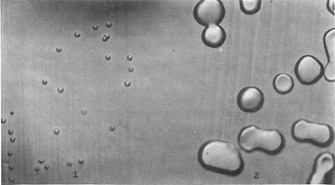
\includegraphics[width=2.5in]{pneumococco r.jpg}
	 	\caption{{\small In questa immagine è possibile osservare le varianti del ceppo R. Sulla sinistra troviamo le cellule cresciute senza esposizione al fattore di trasformazione, mentre sulla destra sono presenti cellule venute in contatto con il fattore.}\cite{o2008isolating}}
	 \end{wrapfigure}
 
	 L'esperimento, che fu realizzato per capire se fosse possibile utilizzare batteri inattivati dal calore come vaccino, consisteva nell'iniezione di due sierotipi del batterio \textit{Streptococcus pneumoniae} :
	 il ceppo rugoso R (dall'inglese \textit{rough}), non virulento e il ceppo liscio S (dall'inglese \textit{smooth}), virulento.
	 Griffith notò che iniettando i ceppi R nelle cavie questi non contraevano malattia, mentre, iniettando i ceppi S, le cavie si ammalavano di polmonite.
	 I batteri S inattivati dal calore invece non erano in grado di indurre patologia a meno che non fossero iniettati insieme a batteri R vivi. Analizzando le colonie batteriche ottenute dai topi infettati da entrambi i ceppi, Griffith scoprì che i batteri del ceppo R si stavano trasformando in quelli del ceppo virulento S. Da questi risultati, Griffith ipotizzò l'esistenza di un \textit{fattore di trasformazione} capace di trasferirsi dalle cellule inattivate S a quelle R, trasformandole.\cite{griffith1928significance}
	 
	 \subsection{La trasformazone batterica}
	 
	 Oltre alla scoperta del \textit{fattore di trasformazione}, con questo esperimento Griffith identificò un nuovo processo biologico, che oggi viene definito \textit{trasformazione batterica}. Questo processo permette a particolari batteri, detti competenti, di assorbire e assimilare catene a doppia elica di DNA esterne alla cellula. Dalla scoperta di questo fenomeno, 82 specie di batteri sono state classificate come essere capaci di ciò, tra cui altri batteri appartenenti alla famiglia dello streptococco, alcuni bacilli e degli attinomiceti tra i batteri Gram-positivi e alcuni batteri Gram-negativi come quelli di genere Chlorobium.\cite{johnston2014bacterial}\\
	 
	 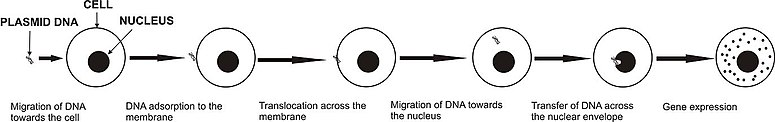
\includegraphics[width=\textwidth]{elettroporazione.jpg}\\
	 
	 Nonostante solo alcuni batteri siano naturalmente in grado di realizzare questo processo, è stato scoperto che la competenza può essere indotta nelle cellule artificialmente in laboratorio. Il primo esempio di ciò risale al 1972, quando Stanley Norman Cohen, Annie Chang e Leslei Hsu dimostrarono che il trattamento con una soluzione di $CaCl_2$ (dicloruro di calcio)  rende competenti le cellule di \textit{Escherichia coli}, batterio fino ad allora considerato refrattario alla trasformazione.\cite{hanahan1983studies} Questa scoperta creò un modo efficiente e conveniente per la trasformazione batterica che permette metodologie di clonazione più semplici nel campo biotecnologico e della ricerca, e che ora è divenuta una delle procedure usate quotidianamente nei laboratori. Inoltre, esiste un'altra procedura di laboratorio in grado di conferire competenza: l'elettroporazione. Essa consiste nell'applicazione di un campo elettrico di migliaia di volt (circa 8kV per 5 $\mu$s) in una cuvetta che contiene cellule e frammenti di DNA in sospensione liquida per incrementare la permeabilità della membrana cellulare, permettendo l'introduzione del materiale genetico. Questo processo, descritto scientificamente per la prima volta nel 1982, divenne il metodo più efficiente, superando di 10 volte i metodi chimici.\cite{neumann1982gene}	
	 
	\section{La scoperta di Avery}
	
	Nonostante le ricerche di Griffith, rimaneva ancora ignota la composizione del \textit{fattore di trasformazione}. Il primo ad identificare la sostanza scoperta da Griffith come DNA fu il medico canadese Oswald Theodore Avery, pioniere della biologia molecolare e dell'immunologia. Mentre il ricercatore inglese si occupava dei suoi esperimenti sui topi, il dottor Oswald e i suoi colleghi della Rockfeller University di New York stavano eseguendo analisi sulle capsule batteriche del pneumococco e sul suo ruolo nelle infezioni, in modo da poter realizzare trattamenti più efficaci per la polmonite batterica. Nel corso degli anni, il team di Avery aveva accumulato considerevole esperienza, dopo aver stabilito di poter distinguere la specie degli pneumococchi attraverso i polisaccaridi contenuti nelle capsule e dopo aver compreso l'importanza dell'integrità della capsula nella virulenza del batterio. Perciò, dopo la pubblicazione delle ricerche di Griffith, Avery e i suoi colleghi compresero l'importanza di queste nuove scoperte e concentrarono la loro attenzione sull'identificazione di specifiche molecole che potessero trasformare un batterio privo di capsula in uno con capsula. Però, a differenza del lavoro di Griffith, Avery utilizzò colonie di cellule al posto di topi, ottenendo maggior controllo sugli esperimenti.
	Avery, con l'aiuto dei suoi colleghi e dei ricercatori Colin MacLeod e Maclyn McCarty, usò il processo dell'eliminazione per identificare il \textit{fattore di trasformazione}.
	
	Nei loro esperimenti, dei campioni identici di cellule del ceppo S trattati col calore sono stati trattati con degli enzimi idrolitici che distruggevano proteine, RNA o DNA. Dopo il trattamento, i campioni trattati sono stati uniti con batteri del ceppo R. Avvenne trasformazione batterica in tutte le colture, tranne quelle in cui le cellule S erano state esposte alla desossiribonucleasi, un enzima che distrugge unicamente il DNA.\cite{avery1944studies} Questi risultati suggerivano che il DNA fosse responsabile della trasformazione, ma i risultati del team di ricerca non furono apprezzati all'epoca, poiché molti membri della comunità scientifica erano ancora convinti che le proteine trasportassero materiale genetico.
	
	\section{Un'ulteriore conferma da parte di Hersey e Chase}
	
	Nonostante lo scetticismo della comunità scientifica, altri ricercatori continuarono a lavorare sull'ipotesi che vedeva il DNA come molecola che trasporta informazioni ereditarie. Tra di essi vie erano i genetisti americani Alfred Hershey e Martha Chase, che, nel 1952, condussero degli esperimenti che supportarono questa ipotesi. Durante le loro ricerche, Hershey e Chase osservarono un batteriofago, virus composto da proteine DNA, infettare dei batteri, in questo caso l'\textit{Escherichia Coli}, identificando il ruolo di ciascuna delle componenti del virus nell'infezione.
	\begin{wrapfigure}{r}{3in}
		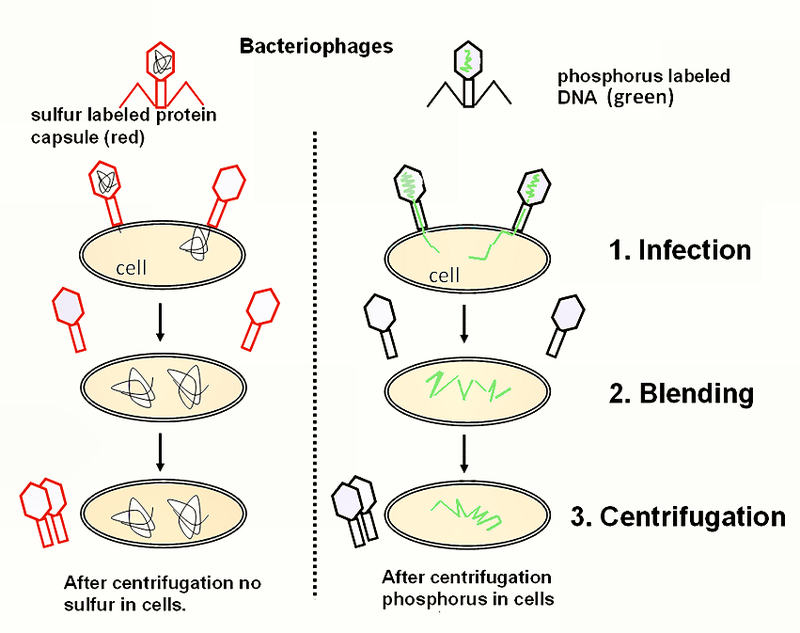
\includegraphics[width=3in]{esperimento-hershey.png}
		\caption{{\small In questa immagine è possibile osservare una schematizzazione dell'esperimento di Hershey e Chase.}}
	\end{wrapfigure}
	 Per fare ciò, i due scienziati avevano bisogno di un modo per distinguere gli elementi del fago e i due decisero di usare degli isotopi radioattivi. Poiché il fosforo è contenuto nel DNA ma non negli amminoacidi, il fosforo-32 fu usato per etichettare il DNA. Al contrario, lo zolfo si può trovare nelle proteine ma non nel DNA, quindi lo zolfo-35 fu utilizzato per distinguere le proteine. Gli isotopi radioattivi furono inseriti nel terreno di coltura dei batteri 4 ore prima dell'esposizione al virus. Dopo l'infezione, la progenie del virus integrò gli isotopi nelle sue strutture. Questo processo fu effettuato per lo zolfo e, successivamente per il fosforo. Dopo il trattamento, i virus marcati infettarono batteri non marcati. Dopo di che, i batteri furono lisi per rilasciare la nuova generazione di virus e la soluzione fu centrifugata per separare le cellule batteriche, più dense, dai fagi, rimasti in sospensione. La progenie dei fagi marcati con il fosforo rimase marcata, evidenziando le trasmissione di materiale genetico, mentre la progenie dei fagi marcati con l'isotopo dello zolfo non presentò alcun tipo di isotopo nelle strutture del virus.\cite{hershey1952independent} Attraverso questo elegante esperimento, Hershey e Chase confermarono ancora una volta che il materiale genetico è contenuto nel DNA. Nonostante ciò, la conferma definitiva del lavoro dei due genetisti americani e dei loro predecessori dovette aspettare ancora una anno, più precisamente il 25 aprile 1953.
	 
	 \section{Watson e Crick: la scoperta della doppia elica}
	 
	La fruttuosa collaborazione tra il biologo statunitense James Dewey Watson e il biofisico britannico Francis Crick iniziò circa un anno e mezzo prima della pubblicazione del loro articolo più famoso. Nell'ottobre del 1951, essi si incontrarono per la prima volta al Cavendish Laboratory, il dipartimento di fisica dell'Università di Cambridge. Dopo questo incontro, i due ricercatori cominciarono a lavorare sulla struttura del DNA: Crick si occupò delle equazioni matematiche che governano la struttura della doppia elica, mentre Watson utilizzò l'esperienza acquisita dal \textit{Phage group}, team di ricerca che si occupava dello studio della genetica attraverso dei batteriofagi. 
	\begin{wrapfigure}{r}{2in}
		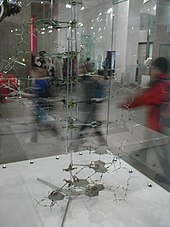
\includegraphics[width=2in]{modelloDNA.jpg}
		\caption{{\small In questa immagine è possibile osservare il modello di DNA originariamente costruito da Watson e Crick, oggi conservato al \textit{Science Museum} di Londra.}}
	\end{wrapfigure}
	Nell'aprile 1952 Watson ebbe l'opportunità di presentare il lavoro svolto fino a quel momento con DNA radioattivo e ricerche che supportavano la presenza di geni negli acidi nucleici. C'è da precisare, però, che il successo dei due scienziati era dovuto anche ad un po' di fortuna: in quell'anno Erwin Chargaff, biochimico austriaco, visitò il Regno Unito e diede importanti chiarimenti a Watson e Crick riguardo ai nucleotidi e, inoltre, Linus Pauling, vicino alla scoperta della struttura, non poté visitare il laboratorio del King's College per motivi politici, ritardando le sue ricerche. Nonostante fu chiesto ai ricercatori di smettere di lavorare sulla struttura del DNA, i due non si diedero per vinti e continuarono a lavorare, sperando di poter ottenere un lavoro simile a quello che Pauling aveva realizzato per le proteine, comprendendone la struttura e le principali interazione con gli enzimi. 
	Però, a differenza di Pauling, Watson e Crick non avevano molta esperienza in campo chimico e si dovettero rivolgere alla chimica e cristallografa britannica Rosalind Franklin, che aveva eseguito diversi lavori sul DNA e che li aiutò nel comprendere molti concetti fondamentali.
	Il 7 marzo del 1953 Watson e Crick realizzano il primo modello di DNA. Esso prevedeva una struttura a doppia elica con catene antiparallele e spiegava anche la complementarità delle basi. Ogni singolo giro di elica era costituito da 10 nucleotidi che quindi potevano trovare spazio su un'intera spira di 360 gradi: l'angolo compreso tra ogni zucchero e il successivo era dunque di 36 gradi. Le basi formavano tra loro legami a idrogeno unendosi alle estremità come tessere del domino. Rompendo i legami a idrogeno la struttura poteva esser aperta come una cerniera e ciò garantiva la duplicazione dei codici.\cite{watson1953molecular} Dopo aver scritto delle loro ricerche in un articolo che sorprendentemente non superò le due pagine, Crick inviò il manoscritto il 2 aprile 1953, che fu successivamente pubblicato dall'autorevole rivista \textit{Nature} il 25 aprile 1953, insieme agli articoli di Wilkins e della Franklin.
	
	\subsection{La vera storia di Rosalind Franklin}
	
	Nonostante sia ben noto che Rosalind Franklin sia stata di grande aiuto a Watson e Crick e che, come Watson stesso la descrive nella sua autobiografia, sia stata una "scienziata ribelle e dai vestiti sobri", la verità è ben diversa. Grazie ai biografi della dottoressa Franklin, sappiamo che quella accusa è totalmente infondata e che i suoi contributi scientifici sono stati molto sminuiti. In verità, Rosalind Elsie Franklin, nata a Londra nel 1920, aveva sempre sognato di diventare una scienziata, che, all'epoca, era molto difficile per una ragazza. Nonostante ciò, con impegno costante e risultati ottimi, ottenne una borsa di studio a Cambridge per laurearsi in chimica e, successivamente, proseguì nei suoi studi per ottenere un dottorato di ricerca. Nel 1951,si unì al King's College per utilizzare la cristallografia a raggi X nello studio della struttura del DNA. Nonostante le sue brillanti ricerche, la comunità scientifica non vedeva ancora di buon occhio le donne e fu sfruttata come un assistente da uno dei suoi colleghi, Maurice Wilkins, che in seguito collaborò con Watson e Crick.
	\begin{wrapfigure}{r}{2in}
		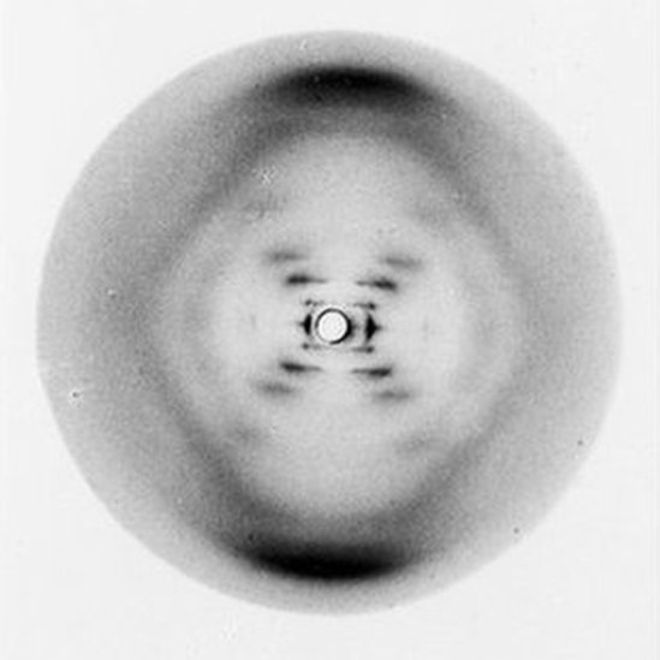
\includegraphics[width=2in]{foto51.jpg}
		\caption{{\small In questa immagine è possibile osservare la famosa foto 51, scattata dalla dottoressa Franklin durante le sue ricerche.}}
	\end{wrapfigure}
	Nonostante ciò, la Franklin continuò a lavorare duramente e, nel 1952, ottenne la celeberrima fotografia 51, immagine ottenuta dall'analisi cristallografica del DNA. Sebbene avesse ottenuto la foto, la Franklin avrebbe avuto bisogno di molto tempo per analizzarla attentamente. Nel frattempo, Watson e Crick ottennero da Wilkins la foto 51 senza il consenso della dottoressa Franklin. I due ricercatori fecero un'analisi sbrigativa dell'immagine della cristallografa e usarono i dati ottenuti per costruire probabili strutture. Alla fine trovarono la famosa doppia elica che oggi conosciamo e pubblicarono i loro risultati nel 1953. Anche la Franklin aveva finito le sue analisi ed era pronta a pubblicare il suo manoscritto. La rivista \textit{Nature} pubblicò entrambi gli articoli, ma pose quello della Franklin per ultimo, facendo sembrare che i suoi esperimenti avessero solo confermato i risultati di Watson e Crick invece di ispirarli. Però, la Franklin aveva già smesso di lavorare sul DNA e morì qualche anno dopo a causa di un cancro, senza mai sapere che Watson e Crick avessero visto i suoi lavori prima della pubblicazione. Watson, Crick e Wilkins vinsero il premio Nobel per la medicina nel 1962 per i loro studi sul DNA. Si dice che anche la Franklin avrebbe vinto il Nobel se solo potessero essere stati assegnati \textit{post mortem}.
	 
	Questa è la vera storia di una donna che ha combattuto il sessismo nella comunità scientifica e che ha rivoluzionato la medicina e la biologia con le sue ricerche.\cite{TedEd2016franklin}
	
	\chapter{La struttura e la composizione degli acidi nucleici}
	
	Sebbene ci volle molto tempo per individuare con precisione le funzioni del DNA, anche prima degli esperimenti di Hershey e Chase, altri ricercatori avevano identificato le molecole che lo costituivano e i legami che li univano. Però, non si conosceva la disposizione tridimensionale del DNA, che è stata successivamente scoperta da Watson, Crick, Wilkins e la Franklin. Oggi, grazie al lavoro svolto sulla struttura degli acidi nucleici, sappiamo decifrare, modificare e ricreare le informazioni trasmesse dal DNA.
	
	\section{La struttura principale}
	
	Il DNA e l'RNA sono macromolecole utilizzate dagli organismi viventi per la conservazione e il trasporto delle informazioni genetiche. Queste molecole sono meglio conosciute come acidi nucleici e sono costituiti da unità ripetitive dette nucleotidi. Questi ultimi sono formati da un gruppo fosfato, uno zucchero pentoso e da una base azotata (adenina, citosina, timina, guanina o uracile). I nucleotidi si legano tra loro attraverso dei \textit{legami fosfodiesterici}, che si forma tra il carbonio $5'$ dello zucchero pentoso e il gruppo fosfato legato al carbonio $3'$ dello zucchero successivo. Da ciò deriva il fatto che alle estremità di ogni filamento di DNA troveremo un gruppo ossidrilico legato al carbonio-$3'$ e un gruppo fosfato legato al carbonio-$5'$. 

	\begin{figure}[h]
	\centering
	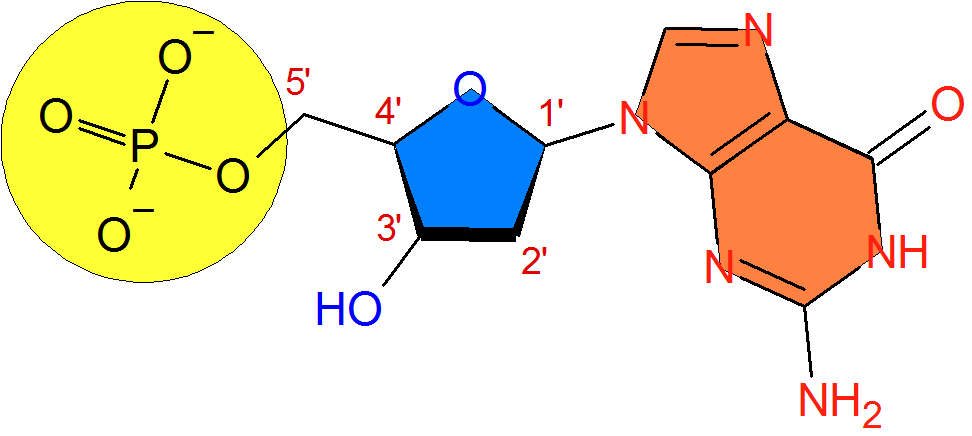
\includegraphics[width=0.7\textwidth]{nucleotideguanina1.png}	
	\caption{{\small In questa immagine è possibile osservare un nucleotide di DNA (deossiguanosina), in cui il gruppo fosfato è evidenziato in giallo, il desossiribosio in blu e la guanina in rosso.}}
	\end{figure}

	Analizzando più attentamente la struttura del nucleotide, scopriamo le singole caratteristiche di ogni componente:\\
	
	Partendo dall'esterno della catena, troviamo il gruppo fosfato, dotato di 2 cariche negative e che conferisce leggera acidità alla macromolecola.\\
	
	Spostandoci verso il centro troviamo lo zucchero pentoso, desossiribosio nel caso  del DNA e ribosio nell'RNA. Questi due zuccheri differiscono solo per un gruppo ossidrilico sul carbonio-$2'$ (il ribosio lo presenta).\\
	
	Infine, troviamo la base azotata, composto che può essere costituito da uno o due anelli principalmente formati da carbonio e azoto. Data la presenza di gruppi amminici, le basi azotate presentano un carattere principalmente basico. Le basi azotate si legano allo zucchero pentoso attraverso un legame N-glicosidico, che come risultato della formazione del legame rilascia acqua. L'unione di una base azotata con lo zucchero forma un nucleoside, che, se fosforato, formerà il nucleotide. Le basi azotate possono essere classificate a seconda della loro struttura: la timina, la citosina e l'uracile si presentano un solo anello e si  definiscono pirimidine, mentre adenina e guanina hanno una struttura a due anelli e sono definiti purine. 
	
	\subsection{Senso}
	
	Una delle caratteristiche più importanti di cui bisogna tenere conto quando si lavora con il DNA è l'orientamento dei filamenti che sono utilizzati. Infatti, le catene sono antiparallele: i due scheletri zucchero-fosfato sono orientati in direzioni opposte ($5' \rightarrow 3'$ e $3' \rightarrow 5'$). Questo concetto è di fondamentale importanza quando si definiscono le posizioni delle strutture a cavallo dei filamenti, come i geni, i fattori di trascrizione, la polimerasi e altri enzimi. Esse sono generalmente definite \textit{a monte} quando si trovano verso l'estremità $5'$ del filamento e \textit{a valle} verso l'estremità $3'$. Il fatto che la sintesi del DNA proceda dal carbonio $5'$ a quello $3'$, ha portato alla convenzione di scrivere e leggere le catene in direzione $5' \rightarrow 3'$\\
	
	L'estremità $3'$ è denominata in questo modo poiché una delle estremità di ogni filamento termina con un gruppo ossidrile in posizione $3'$ che permette la sintesi di nuove molecole di acido nucleico. Per questo motivo, a volte è necessario rimuovere il gruppo -OH per impedire la replicazione; questo processo è noto come \textit{metodo del dideossi}.\\
	
	L'estremità $5'$ è così nominata perché termina con il gruppo fosfato situato presso il carbonio in posizione 5 dell'anello di desossiribosio che rende più difficili i processi di copiatura nei filamenti $3' \rightarrow 5'$. Nonostante ciò, si utilizzano le fosfatasi per rimuovere i fosfati presenti all'estremità $5'$ ed evitare indesiderate ligazioni con altri nucleotidi.
	
	\section{Strutture alternative della doppia elica}
	
	La maggior parte del DNA nelle cellule ha una struttura a spirale destrorsa, presenta basi separate regolarmente ogni 0.36 nm e compie un giro completo ogni 3.6 nm (circa ogni 10.5 coppie di basi per giro). Questa variante di DNA è definita \textit{forma B} ed è la forma più comune osservata negli organismi viventi.\\
	\\
	
	Oltre alla forma B sono stati osservati negli organismi viventi altre due forme di DNA, note come A e Z.\cite{lodish2008molecular}
	
	\begin{wrapfigure}{r}{2in}
		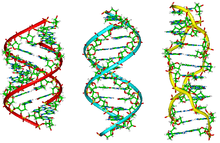
\includegraphics[width=2in]{formeDNA.png}
		\caption{{\small In questa immagine è possibile osservare, a partire da sinistra, le forme di DNA A, B e Z.}}
	\end{wrapfigure}
	
	La forma A è un'ampia spirale destrorsa, con un passo di 2,9 nm (circa 11 paia di basi) ed un diametro di 2,5 nm. Tale conformazione è presente in condizioni non fisiologiche, quando il DNA viene disidratato. In condizioni fisiologiche, questa conformazione caratterizza gli eteroduplex, forme ibride formate da due filamenti provenienti da macromolecole diverse (come nel caso della trasformazione batterica), di DNA.
	
	La conformazione Z è tipica invece delle sequenze che presentano modificazioni chimiche come la metilazione, e dei tratti di DNA ricchi di basi C e G. Essa assume un andamento sinistrorso, opposto rispetto alla conformazione B. Nonostante sia stato identificato in alcune cellule, non si conosce ancora la sua funzione.
	
	\section{Strutture diverse dalla doppia elica}
	
	Le regioni terminali dei cromosomi lineari sono sequenze ripetute dette telomeri. La funzione principale di tali regioni è quella di permettere alla cellula di replicare le estremità dei cromosomi senza che ci sia perdita di informazioni geniche, dal momento che le DNA polimerasi coinvolte nella replicazione del DNA non sono in grado di replicare le estremità 3' dei cromosomi. Nelle cellule umane, i telomeri sono composti da alcune migliaia di ripetizioni di una semplice sequenza costituita da TTAGGG.\cite{wright1997normal}
	Questa sequenza ricca in guanina può stabilizzare le estremità dei cromosomi formando strutture insolite, composte da unità di quattro basi azotate al posto delle canoniche due. Queste strutture sono note con il nome di G-quadruplex, a causa dell'alta concentrazione di guanina nei telomeri. Non si sa ancora molto di queste strutture, ma si sta cominciando ad esplorarle, poiché potrebbero portare a nuove scoperte soprattutto in campo terapeutico, in particolare riguardanti il perfezionamento di farmaci mirati verso i quadruplex di geni specifici.\cite{burge2006quadruplex}
	
	\begin{figure}[h]
		\centering
		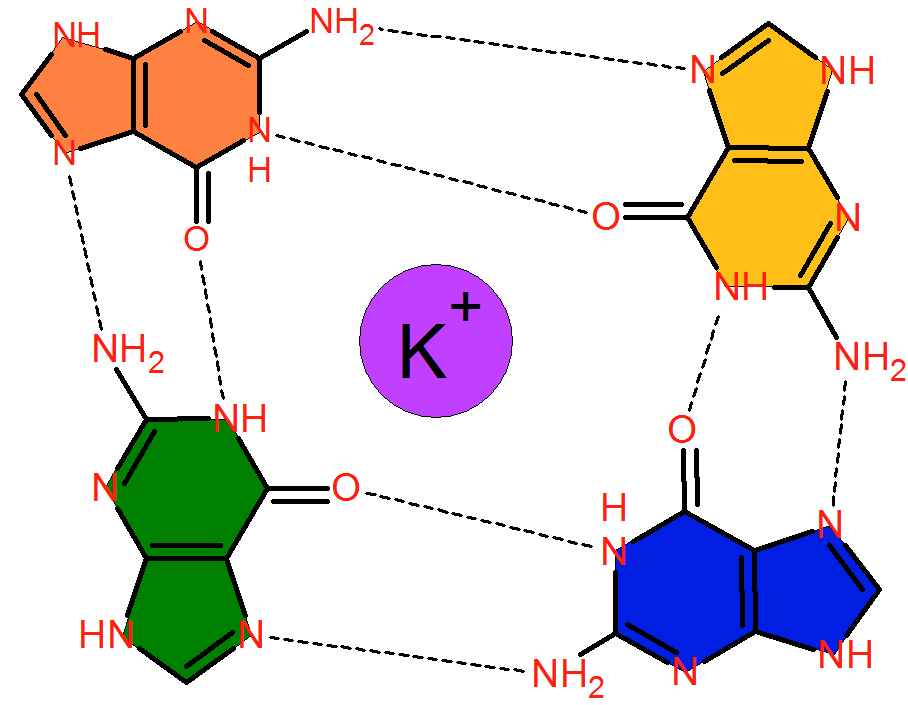
\includegraphics[width=0.47\textwidth]{quadruplex.png}	
		\caption{{\small In questa immagine è possibile osservare la struttura di un G-quadruplex formatosi in presenza di uno ione potassio.}}
	\end{figure}

	\chapter{La replicazione del DNA}
	
	Uno dei temi più importanti della biologia molecolare è sicuramente la duplicazione del DNA, processo di cui già Watson e Crick avevano capito i principi generali. Il regolare appaiamento delle basi nella struttura a doppia elica gli ha suggerito che i nuovi filamenti di DNA fossero sintetizzati partendo dal filamento esistente, usato come stampo. Rimaneva però incerto il modo in cui questo processo avvenisse, poiché erano presenti due possibilità: un meccanismo conservativo e uno semiconservativo. In un meccanismo conservativo, i filamenti figli sarebbero un duplicato del filamento parentale e il filamento parentale stesso. Al contrario, in un meccanismo semiconservativo, il filamento parentale sarebbe diviso per formare due duplicati di se stesso. Prove definitive che il DNA si replica in modo semiconservativo prevengono da un elegante esperimento condotto da M. Meselson e W. F. Stahl.
	
	\section{Esperimento di Meselson e Stahl}
	
	\begin{wrapfigure}{r}{2in}
		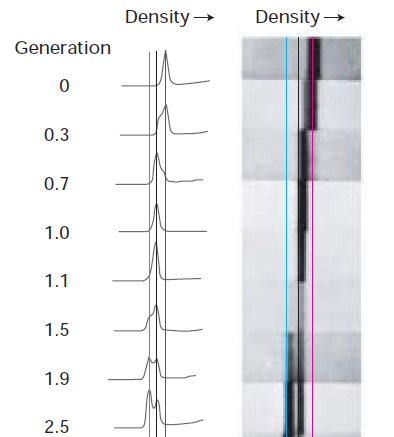
\includegraphics[width=2in]{esperimento-meselson.png}
		\caption{{\small In questa immagine è possibile osservare i risultati delle ricerche di Meselson e Stahl.\cite{lodish2008molecular}}}
	\end{wrapfigure}
	
	Nel loro esperimento, Meselson e Stahl hanno cresciuto delle cellule di \textit{Escherichia coli} in un terreno di coltura contenente sali di ammonio contenenti l'isotopo "pesante" \isotope[15]{N} in modo da marcare tutto il DNA. Dopo che le cellule furono trasferite in un terreno di coltura che contiene il normale e "leggero" isotopo \isotope[14]{N}, alcuni campioni vennero periodicamente rimossi e il DNA fu centrifugato e analizzato secondo il gradiente di concentrazione formato. Questa tecnica permette di separare sezioni di DNA composte da filamenti pesanti-pesanti H-H (dall'inglese \textit{heavy-heavy}), leggeri-leggeri L-L (dall'inglese \textit{light-light}) e pesanti-leggeri H-L (dall'inglese \textit{heavy-light}). Dopo circa 1.9 generazioni, approssimativamente metà del DNA aveva la densità del DNA H-L, mentre l'altra età aveva la densità del DNA L-L. Nelle geerazioni successive, una frazione sempre più grande del DNA estratto consisteva di catene L-L; le catene H-H non comparirono mai. Questi risultati combaciavano con il modello del meccanismo di replicazione semiconservativo, confermando le ipotesi di Watson e Crick sulla replicazione del DNA.\cite{meselson1958replication}\\
	\\
	
	\section{L'inizio della replicazione e lo scopo degli enzimi}
	
	Per fare in modo che il frammento di DNA da duplicare funga da "stampo" per i nuovi filamenti, è necessario che la doppia elica sia svolta affinché possa avvenire l'appaiamento con le basi dei nucleotidi che saranno polimerizzati in nuovi filamenti a doppia elica. La proteina responsabile dello svolgimento del frammento parentale è l'\textit{elicasi}, che comincia ad aprire la doppia elica in specifici segmenti di DNA noti come \textit{origini di duplicazione}, o più semplicemente \textit{ori}. La sequenza di nucleotidi che determina le origini di duplicazione variano da organismo a organismo, anche se sono spesso ricchi di adenina e timina. Dopo la formazione delle origini di duplicazione, un enzima specializzato appartenente alla classe delle RNA polimerasi, la \textit{primasi}, sintetizza un breve molecola di RNA di circa 11 nucleotidi che fungerà da innesco, nota come \textit{primer}. 
	\begin{wrapfigure}{r}{2.5in}
		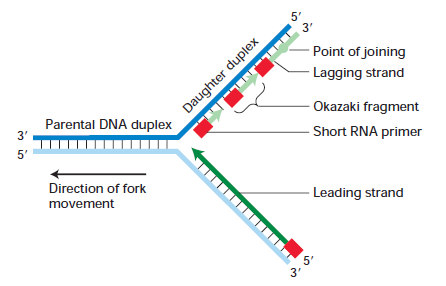
\includegraphics[width=2.5in]{replicazioneDNA.png}
		\caption{{\small In questa immagine è presente una schematizzazione del processo di replicazione.\cite{lodish2008molecular}}}
	\end{wrapfigure}
	Dopo di che, questa breve catena viene allungata da diverse DNA polimerasi (principalmente la \textit{DNA pol III}), così formando il nuovo filamento. La regione di DNA dove tutte queste proteine agiscono è nota come \textit{forcella di duplicazione}. Man mano che la sintesi procede, lo svolgimento della doppia elica causa una torsione nei filamenti a monte della forcella, perciò l'enzima \textit{topoisomerasi I} taglia, gira e riduce i filamenti paternali di DNA ancora non divisi per rimuovere la tensione.
	
	Una delle principali complicazioni incontrate nell'operazione di replicazione nasce da due proprietà della forcella: il fatto che i due filamenti paternali sono antiparalleli e che la DNA polimerasi può aggiungere nucleotidi solo in direzione $5' \rightarrow 3'$. Per questi motivi, la duplicazione procede in modo differente sui due filamenti. Il filamento che presenta l'estremità $3'$ rivolta verso la forcella è noto come \textit{filamento veloce} e può essere replicato senza interruzione. Il filamento antiparallelo, al contrario, viene sintetizzato a ritroso, producendo diversi frammenti alla volta, che richiedono tutti un primer.I segmenti di DNA formati dall'allungamento di questi primer sono detti \textit{frammenti di Okazaki}. Al termine dell'allungamento, l'enzima \textit{DNA ligasi} unirà i frammenti per formare il nuovo filamento e i primer di RNA sono rimossi dalla \textit{DNA pol I}.\\
	
	\section{La replicazione negli eucarioti}
	
	Uno studio dettagliato delle proteine che partecipano nella replicazione del DNA nelle cellule eucariote proviene dalla ricerca condotta sui DNA virali, in particolare il \textit{Simian virus 40}, noto anche come SV40. Nel complesso macchinario specializzato nella replicazione del DNA dell'SV40, una proteina virale detta \textit{antigene-T} svolge la doppia elica nelle origini di duplicazione, formando le forcelle di duplicazione. Tutte le altre proteine utilizzate nella replicazione sono fornite dalla cellula ospite. I primer per il filamento veloce e quello lento sono sintetizzati da un complesso appartenente alla classe delle primasi, che crea un breve filamento di RNA, e da una DNA polimerasi (DNA pol $\alpha$), che estende il primer con deossiribonucleotidi, creando un primer misto, composto da DNA e RNA. Questo primer viene allungato fino a formare un nuovo filamento dalla DNA pol $\delta$, che possiede una minore probabilità di commettere errori durante la replicazione rispetto alla DNA pol $\alpha$. La DNA pol $\delta$ forma un complesso con l'RFC (fattore di replicazione C) e il PCNA (antigene nucleare di proliferazione cellulare), che elimina il complesso primasi-pol $\alpha$ dopo la sintesi del primer. Dopo che il DNA parentale è separato in filamenti singoli, copie della RPA (proteina di replicazione A) si legano ai filamenti, impedendogli di riformare un filamento unico. Queste proteine sono rimosse al passaggio delle DNA pol $\alpha$ e $\delta$ durante la sintesi di nuovi filamenti.\\
	
	\begin{figure}[h]
		\centering
		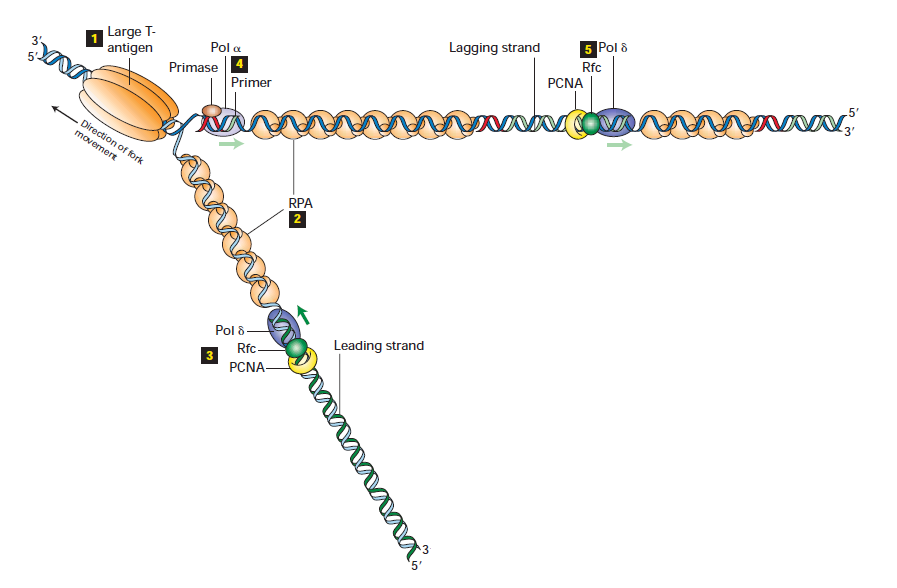
\includegraphics[width=\textwidth]{SV40.png}	
		\caption{{\small In questa immagine è possibile osservare il processo di replicazione del DNA dell'SV40.\cite{lodish2008molecular}}}
	\end{figure}
	
	\section{Correzione degli errori del DNA}
	
	Il processo di duplicazione del DNA permette ad ogni cellula somatica del nostro corpo di possedere lo stesso patrimonio genetico, ma può accadere (circa tra le $10^4$ e le $10^6$ volte al giorno\cite{lodish2008molecular}) che il DNA sia danneggiato. Le cause più frequenti comprendono cause endogene, come un \textit{mismatch}, ovvero un appaiamento di basi sbagliato o l'azione di molecole reattive come il perossido di idrogeno, oppure cause esogene, come l'esposizione a radiazioni, tossine o sostanze mutagene. Per questo motivi, si sono sviluppati alcuni meccanismi di riparazione che eliminano il problema prima che possa causare una mutazione. 
	
	\subsection{Danni ad un singolo filamento}
	
	In molti casi, la parte danneggiata del filamento viene rimossa (escissa) dall'enzima \textit{nucleasi} e viene ripristinato attraverso una DNA polimerasi e una DNA ligasi; questo metodo di riparazione è noto come \textit{riparazione per escissione}. Altri danni comprendono l'ossidazione e l'alchilazione di basi azotate e l'idrolisi di basi, come la depurinazione e la depirimidinazione. Anche le polimerasi sono in grado di correggere i mismatch durante la duplicazione, riducendo i rischi di successive mutazioni. 
	
	\subsection{Danni ad entrambi i filamenti}
	
	Un tipo particolarmente pericoloso di danno al DNA per le cellule in divisione è la rottura di entrambi i filamenti della doppia elica. Esistono due meccanismi capaci di riparare questo danno. Essi sono generalmente conosciuti come \textit{Non-Homologous End-Joining} e \textit{riparazione per ricombinazione}, o ricombinazione omologa.\\
	
	La riparazione per ricombinazione richiede la presenza di una sequenza identica che possa essere usata come "stampo" per la riparazione di una rottura. Il macchinario enzimatico responsabile per questo processo è praticamente identico al macchinario responsabile del crossing-over nelle cellule germinali durante la meiosi.\cite{albert2005principles} Il meccanismo di riparazione per ricombinazione è usato in maniera predominante durante le fasi del ciclo cellulare in cui il DNA si sta replicando o ha completato la duplicazione. Ciò permette ad un cromosoma danneggiato di essere riparato con l'impiego, come "stampo", di un cromatide fratello neosintetizzato. Molti geni nel genoma umano sono presenti in copie multiple fornendo diverse possibili fonti di sequenze identiche.\\
	
	Il Non-Homologous End-Joining (NHEJ) riunisce le due estremità della rottura in assenza di una sequenza che possa fungere da stampo utilizzando enzimi che comprendono DNA-PKcs, Ku, DNA ligasi IV, XRCC4 e altri fattori non ancora identificati. Tuttavia può esserci una perdita di sequenza durante questo processo e quindi tale riparo può essere mutageno. Il NHEJ può verificarsi a tutti gli stadi del ciclo cellulare, ma nelle cellule di mammifero è il principale meccanismo fino a quando la replicazione del DNA non rende possibile la riparazione per ricombinazione con impiego del cromatide fratello come stampo.\cite{mladenov2011induction}
	
	\bibliographystyle{naturemag}
	{\small \bibliography{bibliografiaDNA.bib}}
\end{document}